\chapter{Conceitos Básicos}\label{2-conceitosbasicos}

Nesta seção apresentamos conceitos básicos sobre \textit{grafos, digrafos e complexidade computacional} para explorarmos o problema do \emph{Espectro em convexidade} e outros problemas computacionais. Todos os conceitos abordados aqui foram inspirados nos livros \textit{Introduction to graph Theory}~\cite{west2001introduction}, \textit{Digraphs: Theory, Algorithms and Applications}~\cite{bang2001} e \textit{Introduction to Graph Convexity: An Algorithmic Approach}~\cite{julio}.

\section{Grafos e Digrafos}

Podemos definir um grafo simples da seguinte forma: uma dupla $G=(V,E)$, onde $V(G)$ é o conjunto de vértices do grafo $G$ e $E(G)$ é o conjunto de arestas (pares não ordenados de vértices $vu$ ou $uv$) do grafo $G$. Dizemos que os vértices ligados por uma aresta são suas \emph{extremidades}. Como se trata de grafos simples, não temos \emph{laços}, onde as extremidades de uma aresta são o mesmo vértice e também não temos \emph{arestas múltiplas}, ou seja, duas ou mais arestas compartilham as mesmas extremidades.

Seja $vu \in E(G)$, dizemos então que esses vértices são adjacentes. Denotamos como vizinhança aberta de um vértice $v$, o conjunto de todos os vértices adjacentes a $v$. Quando falamos de vizinhança fechada de $v$, o vértice $v$ também está no conjunto. Com o conceito de vizinhança podemos definir o \emph{grau} de um vértice como $d(v) = |N(v)|$.

Um \emph{caminho} em um grafo $G$, é uma sequência de vértices e arestas em que não há repetição de vértices. Um ($u,v$)-caminho é um caminho em que o primeiro vértice da sequência é $u$ e o último é $v$. Um \emph{ciclo} em um grafo $G$ é um caminho em que o primeiro vértice da sequência é igual ao último. Um grafo é dito \emph{conexo} se para todo par de vértice $u,v \in V(G)$ temos um ($u,v$)-caminho. Seja $H = (V_H,E_H)$, $H$ é um subgrafo de $G=(V,E)$ se $V_H \subseteq V$ e $E_H \subseteq E$. Uma \emph{componente} é um subgrafo maximal conexo de $G$. Uma \emph{ponte} é uma aresta $e \in E(G)$ tal que $G-e$ possui mais componentes que $G$.

Se $G$ é um grafo simples e não contém ciclos, temos que $G$ é uma \emph{floresta}. Uma floresta conexa é chamada de \emph{árvore}. Seja $v \in V(G)$ e $G$ uma floresta (ou árvore), se $d(v) = 1$, dizemos que $v$ é uma folha.

\begin{figure}[ht]
    \centering
    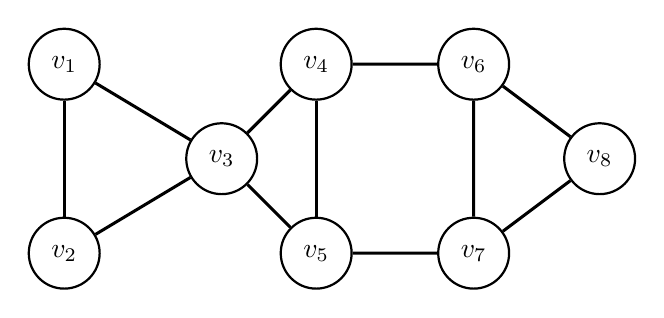
\begin{tikzpicture}[scale=.8,
            vertex/.style={circle, draw, thick, minimum size=0.9cm, font=\normalsize, fill=white},
            aresta/.style={line width=1.1pt}
        ]

        \node[vertex] (v1) at (6,   0)    {$v_8$};
        \node[vertex] (v2) at (4,   1.5)  {$v_6$};
        \node[vertex] (v3) at (1.5, 1.5)  {$v_4$};
        \node[vertex] (v4) at (0,   0)    {$v_3$};
        \node[vertex] (v5) at (1.5, -1.5) {$v_5$};
        \node[vertex] (v6) at (4,   -1.5) {$v_7$};
 
        \node[vertex] (v7) at (-2.5, 1.5)  {$v_1$};
        \node[vertex] (v8) at (-2.5, -1.5) {$v_2$};
 
        \draw[aresta] (v1) -- (v2);
        \draw[aresta] (v2) -- (v3);
        \draw[aresta] (v3) -- (v4);
        \draw[aresta] (v4) -- (v5);
        \draw[aresta] (v5) -- (v6);
        \draw[aresta] (v6) -- (v1);
 

        \draw[aresta] (v3) -- (v5);
        \draw[aresta] (v2) -- (v6);
 

        \draw[aresta] (v4) -- (v7);
        \draw[aresta] (v4) -- (v8);
        \draw[aresta] (v7) -- (v8);

    \end{tikzpicture}
    \caption{Representação de um grafo simples.}\label{fig:peixe}
\end{figure}

Uma \emph{imersão} de um grafo $G$ no plano, é uma função que associa cada vértice de $G$ à um ponto em $\mathbb{R}^2$ e a cada aresta $uv \in E(G)$ a uma $u,v$-curva poligonal simples. A interseção de arestas no plano é um \emph{cruzamento}. Um grafo $G$ é dito \emph{planar} se admite uma imersão no plano $\mathbb{R}^2$ sem cruzamento de arestas.

Um \emph{digrafo} (ou grafo direcionado) é uma dupla $D=(V,A)$, onde $V(D)$ é o conjunto de vértices do digrafo $D$ e $A(D)$ é o conjunto de arcos do digrafo $D$. Diferente das arestas em grafos simples, no contexto dos digrafos, um arco é um par ordenado de vértices. Seja $a=(u,v) \in A(D)$, dizemos que o vértice $u$ é a \emph{cauda} do arco $a$ e o vértice $v$ é \emph{cabeça} do arco $a$. Como temos que os arcos são pares ordenados de vértices, podemos dizer que no arco $(u,v)$, o vértice $v$ é \emph{sucessor} do vértice $u$ e que o vértice $u$ é \emph{predecessor} do vértice $v$. O grafo \emph{subjacente} de $D$ é o grafo sem as orientações dos arcos. 

Neste texto, quando falarmos grafos, estamos nos referindo à grafos simples, e grafos orientados, à digrafos com grafo subjacente sendo um grafo simples. Dado um grafo $G$, a orientação de $G$ é atribuir para cada aresta $e=uv \in E(G)$ uma única orientação, $(u,v)$ ou $(v,u)$. Se o grafo $G$, é um \emph{grafo completo}, ou seja, para cada par de vértices $u,v \in V(G)$, temos uma aresta, ao orientarmos $G$, obtemos um \emph{torneio}.

Os conceitos de caminhos e ciclos também existem no contexto orientado, basicamente ao invés de termos arestas, temos arcos, vale ressaltar que um ($u,v$)-caminho orientado não significa que temos um ($v,u$)-caminho orientado. O grafo orientado $D$ é conexo, se o grafo subjacente de $D$ é conexo. Dizemos que o grafo orientado é \emph{fortemente} conexo se para todo par de vértices $u,v \in V(D)$ existe um ($u,v$)-caminho orientado e um ($v,u$)-caminho orientado.

Se o arco tem as extremidades no mesmo vértice, temos um \emph{laço}, os \emph{arcos múltiplos} são dois ou mais arcos que compartilham a mesma \emph{cabeça} e \emph{cauda}. Se temos laços e arcos múltiplos, se trata de um \emph{pseudodigrafo}, quando temos apenas arcos múltiplos, se trata de um \emph{multidigrafo}. Também podemos dizer que um digrafo sem laços e sem arcos múltiplos é um grafo orientado.

Assim como nos grafos não orientados, o conceito de vizinhança se mantém, mas nesse caso, se divide em \emph{vizinhança de entrada} e \emph{vizinhança de saída}. Seja $v \in V(D)$, a vizinhança de entrada de $v$, denotado por $N^-(v)$, é o conjunto de todos os predecessores de $v$, já a vizinhança de saída de $v$, denotado por $N^+(v)$, é o conjunto de todos os sucessores de $v$. Com isso, podemos definir \emph{grau de entrada} de $v$ como $d^-(v) = |N^-(v)|$ e \emph{grau de saída} de $v$ como $d^+(v)=|N^+(v)|$.

\begin{figure}[ht]
	\centering
	\begin{tikzpicture}[scale=.8,
            vertex/.style={circle, draw, thick, minimum size=0.9cm, font=\normalsize},
            arco/.style={-{Latex[length=1.5mm, width=2.4mm]}, line width=1.1pt},
            branco/.style={fill=white},
            cinza/.style={fill=gray!40, draw=gray!70!black},
            azul/.style={fill=blue!20, draw=blue!60!black},
            vermelho/.style={fill=red!30, draw=red!70!black}
        ]
	
            \node[vertex, branco] (v1) at (0, 2) {$v_1$};
            \node[vertex, branco] (v2) at (0, 0) {$v_2$};
            \node[vertex, branco] (v3) at (2.2, 1) {$v_3$};
            \node[vertex, branco] (v4) at (4.4, 0) {$v_4$};
            \node[vertex, branco] (v5) at (4.4, 2) {$v_5$};
            \node[vertex, branco] (v6) at (6.6, 1) {$v_6$};
 
            \draw[arco] (v1) -- (v3);
            \draw[arco] (v3) -- (v2);
            \draw[arco] (v4) -- (v2);
            \draw[arco] (v3) -- (v4);
            \draw[arco] (v1) -- (v5);
            \draw[arco] (v5) -- (v3);
            \draw[arco] (v6) -- (v4);
            \draw[arco] (v5) -- (v6);

	\end{tikzpicture}
	\caption{Uma representação de um grafo orientado $D$.}\label{fig:digrafo}
\end{figure}

\section{Complexidade Computacional}

Além dos resultados de convexidade mais estruturais, este trabalho apresenta resultados em complexidade computacional. Existem várias classes de complexidade, mas vamos focar em apenas duas: \poli~e~\np. Para melhor entendimento desses conceitos, recomenda-se a leitura de~\cite{garey1990} e de~\cite{cormen2012algoritmos}.

Em~\cite{cormen2012algoritmos}, vemos que um \emph{algoritmo} é qualquer procedimento computacional bem definido que toma algum conjunto de valores como \emph{entrada} e produz um conjunto de valores como saída. Um \emph{problema computacional} é um problema que relaciona um conjunto de entrada com um conjunto de saída. Portanto, um algoritmo é um conjunto de etapas para resolver um problema computacional. Um \emph{problema de decisão} é uma pergunta com resposta \emph{sim} ou \emph{não} sobre algum parâmetro de entrada de um problema computacional.

\subsection{Classes de complexidade}

A classe~\poli~é definida como o conjunto de todos os problemas de decisão que podem ser resolvidos por algoritmos polinomiais. Um \emph{verificador polinomial} é um algoritmo que dada uma instância de um problema em que a resposta é sim, e um \emph{certificado} de tamanho polinomial, checa se a resposta para a instância do problema realmente é \emph{sim}, ou seja, o verificador retorna \emph{sim} se e somente se a resposta da instância é \emph{sim}. A classe NP é basicamente a classe para os problemas de decisão que possuem um verificador polinomial para \emph{sim}. Quando falarmos nesse texto de algum problema computacional, entende-se que se trata de um problema de decisão.

Sejam $A$ e $B$ dois problemas distintos. Uma \emph{redução polinomial} entre problemas é um algoritmo de tempo polinomial $f$ que transforma uma instância $I$ de $A$ em uma instância $f(I)$ de $B$. Neste caso, a instância $I$ de $A$ tem resposta \emph{sim}, se e somente se, a instância $f(I)$ de $B$ tem resposta \emph{sim}. Dizemos que um problema $A$ é~\npd, se todo problema da classe~\np, pode ser reduzido em tempo polinomial ao problema $A$. Por fim, dizemos que um problema $A$ é~\npc~se $A$ está em~\np~e também é um problema~\npd. Observe que dessa forma, todo problema~\npc~pode ser reduzido em tempo polinomial para outro problema~\npc.